\section{Experiments}
\label{sec:experiments}

\myparagraph{Implementation details}
We employ SAM2 with Hiera-Large \cite{ryali2023hiera} as encoder. AdaptFormer \cite{chen2022adaptformer} is inserted into the last two blocks, with hidden size set to $0.3\times$ the block channel dimension in the strict few-shot setting and $0.8\times$ in the generalist. \sam{} is frozen, and \textbf{only the adapters are trained} ($\sim$10M params in the strict case and $\sim$25M in the generalist). We train with AdamW and learning rate $10^{-4}$ for 5 epochs (strict) and 20 (generalist), with $k{=}1$ (a single annotated reference) and sequence length $J{=}3$. The same model is evaluated on 1-shot and 5-shot. Full details are in~\cref{sec:supp_implementation}.






\myparagraph{Datasets}
\textbf{COCO-20$^i$} \cite{nguyen2019feature} is built on MSCOCO \cite{lin2014microsoft} and consists of 80 classes split into four folds, each with 20 classes. 
\textbf{FSS-1000} \cite{gao2022mutually} contains 1000 classes, with 520 for training, 240 for validation, and 240 for testing.
\textbf{LVIS-92$^i$} \cite{liu2023matcher} is more challenging, selecting 920 classes from LVIS \cite{gupta2019lvis}, divided in 10 folds. 
\textbf{PASCAL-Part} \cite{liu2023matcher} includes four superclasses with 56 object parts across 15 classes.
\textbf{PACO-Part} is built from PACO \cite{ramanathan2023paco} and contains 303 classes, split in four folds. 

\subsection{Strict Few-Shot Segmentation Setting}

We first evaluate our method in strict FSS setting. Following standard protocols \cite{wang2023amf, sun2024vrp, shi2022dense}, we train on base classes and evaluate on \textbf{novel} classes with \textit{k}-shots. These experiment address the question of whether the \textit{semantic mapping} learned on base classes can transfer meaningfully to novel categories. 


\begin{table*}
\begin{center}
\setlength{\tabcolsep}{2pt}
\caption{\textbf{Strict Few-Shot Segmentation setting}. Results for $k$-shot segmentation on LVIS-92$^i$, COCO-20$^i$, and FSS-1000. We include both specialist models and approaches based on foundation models, trained and tested on disjoint classes. Training-free methods are also reported for reference.}
\begin{adjustbox}{width=0.9\linewidth}
\begin{tabular}{llcr|cc|cc|cccccccc}
\toprule
\multirow{3}{*}{Method} & \multirow{3}{*}{Venue} & \multirow{3}{*}{Backbone} & \multirow{3}{*}{Params} & \multicolumn{6}{c}{\emph{few-shot segmentation}} \\
& & & & \multicolumn{2}{c|}{LVIS-92$^i$} & \multicolumn{2}{c|}{COCO-20$^i$} & \multicolumn{2}{c}{FSS-1000} \\
& & & & 1-shot & 5-shot & 1-shot & 5-shot & 1-shot & 5-shot  \\
\midrule 
\multicolumn{2}{l}{\emph{Training-free methods}} & &&&&&& \\
~~SAM 2 \cite{ravi2024sam} & \puB{-} & \scriptsize{SAM2-L} &  224 M & 16.5 & 26.3 & 32.2 & 44.2 & 73.0 & 84.3 \\
~~PerSAM \cite{zhang2023personalize} & \puB{ICLR'24} & \scriptsize{SAM-H} & 641 M &  11.5 & - & 23.0 & - & 71.2 & -  \\
~~Matcher \cite{liu2023matcher} & \puB{ICLR'24} & \scriptsize{DINOv2-L+SAM-H} &  945 M & 33.0 & 40.0 & 52.7 & 60.7 & 87.0 & 89.6  \\
~~GF-SAM \cite{zhang2024bridge} & \puB{NeurIPS'24} & \scriptsize{DINOv2-L+SAM-H} & 945 M & 35.2 & {44.2} & {58.7} & {66.8} & 88.0 & 88.9  \\
\midrule

\multicolumn{2}{l}{\emph{Strict $k$-shot segmentation}} &&&&&& \\
~~AMFormer \cite{wang2023amf} & \puB{NeurIPS'23} & \small{ResNet101} & 49 M & - & - & 51.0 & 57.3 & - & -  \\
~~HMNet \cite{xu2025hybrid} &\puB{NeurIPS'24} & \small{RN50} & 39 M & - & - & 52.1 & 58.9 & - & -  \\
~~VRP-SAM \cite{sun2024vrp} & \puB{CVPR'24} & \small{RN50 + SAM-H} & 670 M &  28.3 & - & 53.9 & - & 87.7 &  - \\
~~SegIC \cite{meng2024segic} & \puB{ECCV'24} & \small{DINOv2-G} & 1.2 B & {40.5} & - & 53.6 & - & 88.5 & -  \\

~~DiffewS \cite{zhu2024unleashing} & \puB{NeurIPS'24} & \small{StableDiffusion} & 890 M & 33.9 & {43.7} & 52.2 & 60.7 & 90.2 & 90.6  \\
~~\textbf{\ours{}} & \puB{NeurIPS'25} & \small{SAM2-L} & 234 M & \textbf{48.8} & \textbf{53.9} & \textbf{60.2} & \textbf{64.3} &   \textbf{91.4} & \textbf{92.1}   \\
\bottomrule
 
\end{tabular}
\label{tab:strict_few_shot}
\end{adjustbox}
\end{center}
\vspace{-0.5cm}
\end{table*}



\myparagraph{Few-shot segmentation}
In \cref{tab:strict_few_shot}, we compare \ours{}, besides specialist models, such as AMFormer \cite{wang2023amf} and HMNet \cite{xu2025hybrid}, with the most relevant and recent approaches based on Foundation Models. These include methods that, like ours, leverage a single Foundation Model, such as SegIC \cite{meng2024segic} and DiffewS \cite{zhu2024unleashing}, as well as modular two-stage pipelines like VRP-SAM \cite{sun2024vrp}. For completeness, we also report results from generalist \textit{training-free} methods built on DINOv2 and SAM, including PerSAM \cite{zhang2023personalize}, Matcher \cite{liu2023matcher}, GF-SAM \cite{zhang2024bridge}, as well as our baseline, \textit{i.e.} frozen \sam{}.


In the one-shot setting, \ours{} consistently outperforms all prior methods, demonstrating superior generalization to unseen classes. Specifically, we surpass the best direct competitors SegIC, VRP-SAM and DiffwS by +8.3\%, +6.3\%, and +1.2\% on LVIS-92$^i$, COCO-20$^i$, and FSS-1000, respectively. This performance gap remains consistent also against training-free approaches: compared to GF-SAM, \ours{} achieves gains of +13.6\%, +1.5\%, and +3.4\%.
On the challenging LVIS-92$^i$, including 920 fine-grained categories (e.g., \textit{bulldog}, \textit{dalmatian}), DINO-based methods (SegIC, GF-SAM, Matcher) tend to underperform, possibly due to DINO overly-semantic features \cite{engstler2023understanding, zhang2023tale} (\textit{e.g.}, grouping distinct breeds  under the concept of “dog”). Here, \ours{} achieves a substantial +8.3\% gain, suggesting that \sam{} encodes a latent hierarchical semantic structure, capturing both high-level semantic concepts (dominant in COCO-20$^i$) and fine-grained distinctions (crucial for LVIS-92$^i$). 

Regarding the 5-shot setting, we note that SegIC and VRP-SAM do not provide an inference pipeline to extend to $k$-shot. In contrast, \ours{} natively models correspondences across multiple reference frames and it outperforms the best competitor, DiffewS, by +10.2\% and +3.6\% on LVIS-92$^i$ and COCO-20$^i$, respectively. Compared to training-free models, SANSA shows improvements of +9.7\%, +3.2\%, on LVIS-92$^i$ and FSS-1000, while suffering a -2.5\% gap on COCO-20$^i$ w.r.t. GF-SAM.
We also report results of upgrading SAM-based baselines to SAM2 in \cref{sec:supp_backbone}.

\begin{figure*}[t]
\centering
% === LEFT SIDE ===
\begin{minipage}{0.47\textwidth}
    \centering
    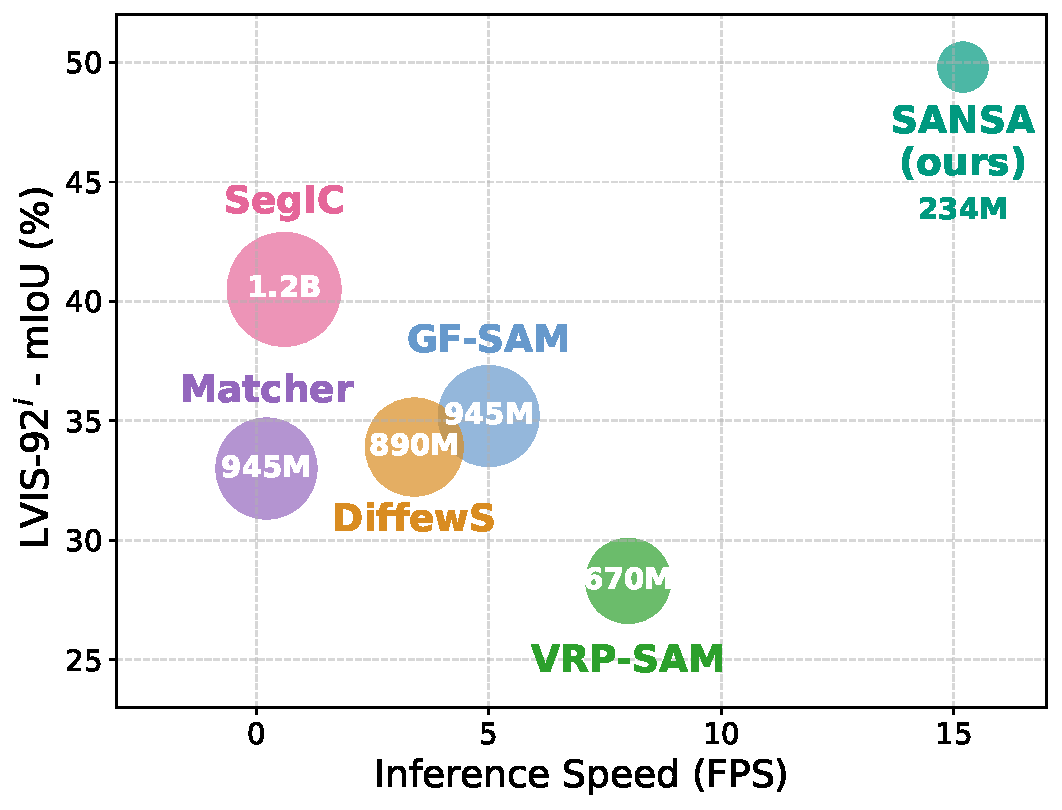
\includegraphics[width=\textwidth]{images/miou_vs_fps.pdf}
    \vspace{-15pt}
    \captionof{figure}{\textbf{Comparison of inference speed and mIoU}, with bubble size representing \#parameters. The plot highlights our superior trade-off.}
    \label{fig:fps_new}
\end{minipage}
\hspace{8pt}
% === RIGHT SIDE  ===
\begin{minipage}{0.49\textwidth}
    
    \setlength\tabcolsep{2.5pt}
    \centering
    \begin{adjustbox}{width=0.65\textwidth}
    \begin{tabular}{l|ccc}
      & VRP-SAM & \multicolumn{2}{l}{\textbf{\ours{}(ours)}}  \\
    \toprule
    Params   & 670M & 234M & \\
    \toprule
    \emph{point}    & 38.4 & 53.4 & {\footnotesize\textcolor{black!60}{+15.0}} \\ 
    \emph{scribble} & 47.3 & 53.1 & {\footnotesize\textcolor{black!60}{+5.8}} \\
    \emph{box}      & 49.7 & 54.3 & {\footnotesize\textcolor{black!60}{+4.6}} \\
    \emph{mask}     & 53.9 & 60.2 & {\footnotesize\textcolor{black!60}{+6.3}} \\
    \bottomrule
    \end{tabular}
    \end{adjustbox}
    \vspace{0.1cm}
    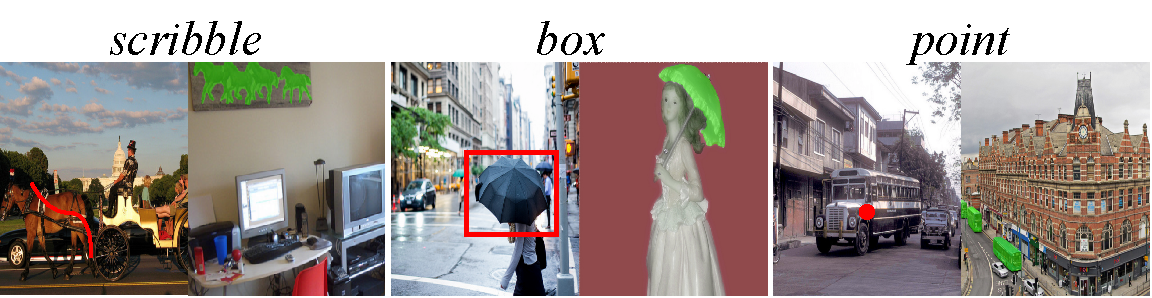
\includegraphics[width=\textwidth]{images/promptable.pdf}
    \caption{\textbf{Promptable few-shot segmentation with \ours{}.} Top: performance in strict few-shot (COCO-20$^i$) using different prompt types compared with VRP-SAM. Bottom: qualitative examples with point, scribble, and box prompts.}
    \label{fig:promptable_combined}
\end{minipage}

\end{figure*}


\myparagraph{Performance-Efficiency Trade-off}
In \cref{fig:fps_new}, we analyze the trade-off between model size, inference speed (img/s), and performance. \ours{} achieves state-of-the-art results while being the most lightweight solution. Specifically, it is: \textit{i)} over 3× faster than the direct competing method (GF-SAM), \textit{ii)} more compact, introducing only adapter parameters on top of \sam{} (totaling 234M), and \textit{iii)} substantially more accurate, outperforming GF-SAM by +13.6\% mIoU on the challenging LVIS-92$^i$ benchmark.
Importantly, \ours{} keeps the SAM2 architecture entirely frozen, meaning that by storing only the adapter weights, it retains \sam{} state-of-the-art performance on Video Object Segmentation while also achieving top-tier results on few-shot segmentation within a single model. A large-scale annotation study quantifying speed/quality trade-offs is presented in~\cref{sec:supp_scalable}.


\myparagraph{One-Shot Promptable Segmentation}
Our framework keeps \sam{} decoder frozen, maintaining its capability to generate masks from any prompt (\ie points, scribbles, or boxes). As such, during inference, users can segment reference objects by providing a simple point, without requiring costly pixel-level masks. In \cref{fig:promptable_combined} we evaluate the performance with different prompts on strict FSS setting on COCO-20$^i$ against VRP-SAM, which also supports such prompts.
\ours{} shows gains of +15.0\%, +4.6\%, and +5.8\% when using points, scribbles, and boxes as annotations. More importantly, the performance drop from masks to point prompts is substantially smaller for \ours{} (-6.8\%) compared to VRP-SAM (-15.5\%). We attribute this to the tightly coupled design of our architecture, which maximizes feature reuse by jointly leveraging the same representations for prompt encoding, feature matching, and mask decoding. Prompt generation details and qualitative results are in~\cref{sec:supp_qualitative}.



\subsection{Generalist In-Context Setting}
\label{sec:in_context}

Following recent few-shot segmentation works \cite{meng2024segic, zhu2024unleashing, liu2023matcher, zhang2024bridge}, we evaluate \ours{} in the in-context segmentation setting, where a single generalist model is tested across multiple benchmarks (\textit{cf}. \cref{tab:main_table_generalist}). Given the lack of a standardized training protocol, we explicitly report additional datasets used by each method beyond ADE20K and COCO, which are shared across all approaches.
We evaluate three configurations of our approach: \textit{i)} a minimal setup using only COCO and ADE20K, \textit{ii)} an extended version incorporating LVIS, following the setup of SegIC \cite{meng2024segic}, and \textit{iii)} a variant including PACO to mitigate object-level bias and reinforce part segmentation capabilities.



When trained only on COCO and ADE20K coarse categories, \ours{} exhibits strong out-of-domain generalization on the LVIS benchmark, outperforming DiffewS and SINE by +4.8\% and +5.0\%, respectively. Moreover, when LVIS is included in the training set (matching SegIC in-domain setup), \ours{} further improves performance and surpasses SegIC by +5.4\%.
Despite not being trained at the part level, \ours{} exhibits strong cross-task generalization capabilities, surpassing generalist baselines by a large margin (+7.5\% and +8.4\% over DiffewS, the best competitor on Pascal-Part and Paco-Part, respectively), including those trained on part segmentation datasets \cite{wang2023seggpt, liu2024simple}. Our method is only outperformed by training-free models, which, by design, are not biased by object-level training. To address this bias, we follow \cite{wang2023seggpt, liu2024simple} and augment our training set with PACO, leading to +6.7\% on Paco-Part (in-domain) and +4.6\% on Pascal-Part (out-of-domain) against the strong baseline of GF-SAM. Finally, we highlight that, within the generalist model category, \ours{} is the most compact solution, with only 250 M parameters.

\begin{table*}
\begin{center}
\caption{\textbf{Performance of \ours{} against Generalist In-context models}. Excluding training-free approaches, all methods are trained on COCO and ADE20k, and we report additional training datasets for each one.  SegIC (*) uses additional supervision via a textual meta-prompt at test time.}
\label{tab:main_table_generalist}
\begin{adjustbox}{width=.96\linewidth}
\setlength\tabcolsep{4pt}
\begin{tabular}{lcr|cc|cc|cc|cc}
&&&  \multicolumn{6}{c|}{\emph{few-shot segmentation}} & \multicolumn{2}{c}{\emph{part seg.}} \\
\multirow{2}{*}{Method} & \multirow{2}{*}{\begin{tabular}[c]{@{}c@{}} Additional \\ Datasets \end{tabular}} & \multirow{2}{*}{Params} & \multicolumn{2}{c|}{LVIS-92$^i$} & \multicolumn{2}{c|}{COCO-20$^i$} & \multicolumn{2}{c|}{FSS-1000} & Pascal & PACO \\
& & & 1-shot & 5-shot & 1-shot & 5-shot & 1-shot & 5-shot & Part & Part \\
\midrule 
\multicolumn{3}{l|}{\emph{Training-free methods}} &&&&&&& \\
~~Matcher \cite{liu2023matcher} & \textit{n.a.} & 945M  & 33.0 & 40.0 & 52.7 & 60.7 & 87.0 & 89.6 & 42.9 & 34.7 \\
~~GF-SAM \cite{zhang2024bridge} & \textit{n.a.} & 945M & 35.2 & 44.2 & {58.7} & {66.8} & 88.0 & 88.9  &  {44.5} & {36.3} \\
\midrule
~~Painter \cite{wang2023images} & \makecell{NYUv2} & 354 M  & 10.5 & 10.9 & 33.1 & 32.6 & 61.7 & 62.3 & 30.4 & 14.1 \\
~~SegGPT \cite{wang2023seggpt}  & \makecell{Pascal, PACO} & 354 M  & 18.6 & 25.4 & 56.1 & 67.9 & 85.6 & 89.3 & 35.8 & 13.5 \\
~~SINE \cite{liu2024simple}  & \makecell{Object365, PACO} & 373 M  & 31.2 & 35.5 & 64.5 & 66.1 & - & - & 36.2 & - \\
~~DiffewS \cite{zhu2024unleashing}  & \makecell{Pascal} & 890 M  & 31.4 & 35.4 & 71.3 & 72.2 & 87.8 & 88.0 & 34.0 & 22.8 \\
~~SegIC \cite{meng2024segic}  & \makecell{LVIS} & 1.2 B  & 47.8 & - & {74.5*} & - & 88.4 & - & 31.2 & 18.7 \\
\midrule
~~\textbf{\ours} & - & 250 M  & 36.2 & 42.5 & \textbf{76.4} & {77.1} & 88.2 & 89.0 & 40.4 & 29.2 \\
~~\textbf{\ours} & \makecell{LVIS} & 250 M  & \textbf{53.2} & {58.1} & {74.7} & {76.3} & {89.1} & {89.7} & {41.5} & {31.2} \\
~~\textbf{\ours} & \makecell{LVIS, PACO} & 250 M  & {50.3} & \textbf{59.0} & {75.6} & \textbf{78.6} & \textbf{90.0} & \textbf{91.0} & \textbf{49.1} & \textbf{43.0} \\
\bottomrule
\end{tabular}
\end{adjustbox}
\end{center}
\vspace{-0.5cm}
\end{table*}

\subsection{Generalization across domains and styles}
To explore how \ours{} generalizes beyond the scope of standard benchmarks, we follow \cite{sun2024vrp, liu2023matcher} and present qualitative examples drawn from in-the-wild image pairs, shown in \cref{fig:wild}. In each case, the model is tasked with few-shot segmentation using a reference image from COCO \cite{lin2014microsoft} and a target image collected from the web, offering a complementary view to benchmark evaluations.

\begin{figure}[h]
    \centering
    \includegraphics[width=0.95\linewidth]{images/wild.pdf}
    \caption{\textbf{Few-shot segmentation with SANSA in-the-wild}. These examples showcase \ours{} ability to handle alternative types of challenges not typically covered by standard benchmarks, such as domain shifts (\textit{e.g.}, real-world to cartoon) and style variations (\textit{e.g.}, photos to sketches).}
    \label{fig:wild}
\end{figure}

These examples introduce a different challenge compared to traditional benchmarks, focusing on domain and style shifts, such as when the target image is a cartoon or stylized sketch, or when the visual appearance changes dramatically between the reference and target. These results demonstrate \ours{} strong generalization. Importantly, this robustness across domains and styles is inherited from the frozen \sam{}. Our method preserves this capability by learning a semantic mapping within the frozen feature space, enabling reliable correspondence even under significant distribution shifts.

\subsection{Ablation studies}
\begin{table}[t]
\centering
\caption{Ablation on COCO-20$^i$. 
\textbf{Left:} fine-tuning underperforms adaptation. 
\textbf{Middle:} simple adapters yield strong gains, while higher capacity (larger bottlenecks or added complexity, \textit{e.g.}, MONA) hurts generalization.
\textbf{Right:} adapting the last two stages suffices to disentangle semantics.}
\vspace{5pt}
\label{tab:ablations}
\setlength{\tabcolsep}{6pt} % default is 6pt, increase spacing
\resizebox{0.95\linewidth}{!}{%
\begin{tabular}{lrc|lc|lcc}
\toprule
\multicolumn{3}{c|}{\textbf{Fine-tuning strategies}} & 
\multicolumn{2}{c|}{\textbf{Adaptation strategies}} &
\multicolumn{3}{c}{\textbf{Adapter placement}} \\
\cmidrule(lr){1-3} \cmidrule(lr){4-5} \cmidrule(lr){6-8}
\textbf{Method} & \textbf{Params} & \textbf{mIoU} &
\textbf{Method} & \textbf{mIoU} &
\textbf{Stages} &  & \textbf{mIoU} \\
\midrule
Frozen & 0 & 32.2 & LoRA \cite{hu2022lora} & 58.0 & None & – & 32.2 \\
From Scratch & 224 M & 37.1 & Adapter \cite{houlsby2019adapter} & 59.4 & All & 0–3 & 59.4 \\
Full FT & 224 M & 51.6 & MONA \cite{yin20255} & 56.9 & Early & 0–1 & 38.7 \\
Decoder FT & 4 M & 52.1 & AdaptFormer \cite{chen2022adaptformer} &  & Middle & 1–2 & 57.9 \\
QKV FT & 50 M & 55.3 & \;\;Bottleneck $0.8\times$ channel dim & 58.2 & Late & 2–3 & \textbf{60.2} \\
Backbone FT & 210 M & 55.2 & \;\;Bottleneck $0.5\times$ channel dim & 59.6 &  &  &  \\
SANSA & 10 M & \textbf{60.2} & \;\;Bottleneck $0.3\times$ channel dim & \textbf{60.2} &  &  &  \\
\bottomrule
\end{tabular}%
}
\setlength{\tabcolsep}{6pt} % reset to default after table
\end{table}


We investigate three central aspects of our design: adaptation vs.\ fine-tuning, adapter architecture and capacity, and adapter placement. Results are summarized in \cref{tab:ablations}.

\textbf{Why adaptation instead of fine-tuning?} A central question of our work is how to distill knowledge from a pretrained model (\textit{i.e.}, \sam{}) while preserving generalization, a key challenge in FSS.
To this end, we evaluate fine-tuning strategies targeting the decoder, QKV projections, backbone, and full model, and compare them with inserting adapters into frozen weights. Results show that adaptation outperforms fine-tuning, indicating that it better preserves \sam{} pretrained priors, shifting the embedding space toward task-relevant semantics without altering the underlying representations. 

\textbf{What makes an adaptation strategy effective?}  
Basic adapters such as LoRA~\cite{hu2022lora}, Adapter~\cite{houlsby2019adapter}, and AdaptFormer~\cite{chen2022adaptformer} all yield similar gains around $\sim$27\% mIoU over frozen \sam{}. The slight gains ($\sim$2\%) with Adapter and AdaptFormer w.r.t. LoRA suggest that a simple non-linearity can refine this structure but not fundamentally reshape it. By contrast, increasing adapter capacity, either by enlarging the bottleneck or using more complex designs such as MONA~\cite{yin20255}, reduces generalization. These results show that effective adaptation thus requires simplicity and constraint: low-capacity, bottlenecked modules best expose \sam{} latent semantics, while excessive capacity tends to overfit.


\textbf{Where should adapters be placed?}  
Prior works often insert adapters throughout the entire backbone. In our case, we find that adapting only the last two stages is sufficient, as these layers already capture high-level semantic information, which is the focus of our disentanglement objective.

Additional ablations, including backbone scale and training objective, are provided in~\cref{sec:supp_backbone}.



